L'analisi esplorativa è stata effettuata sull'intero dataset ripulito. 
L'esplorazione dei dati è stata eseguita utilizzando il package R 
\textbf{DataExplorer} e tramite il software \textbf{Power BI}.

Il primo passo è stato visualizzare la distribuzione di colonne con valori 
continui, discreti e mancanti, utilizzando la funzione \texttt{plot\_intro}.

\begin{figure}[htb]
	\centering
	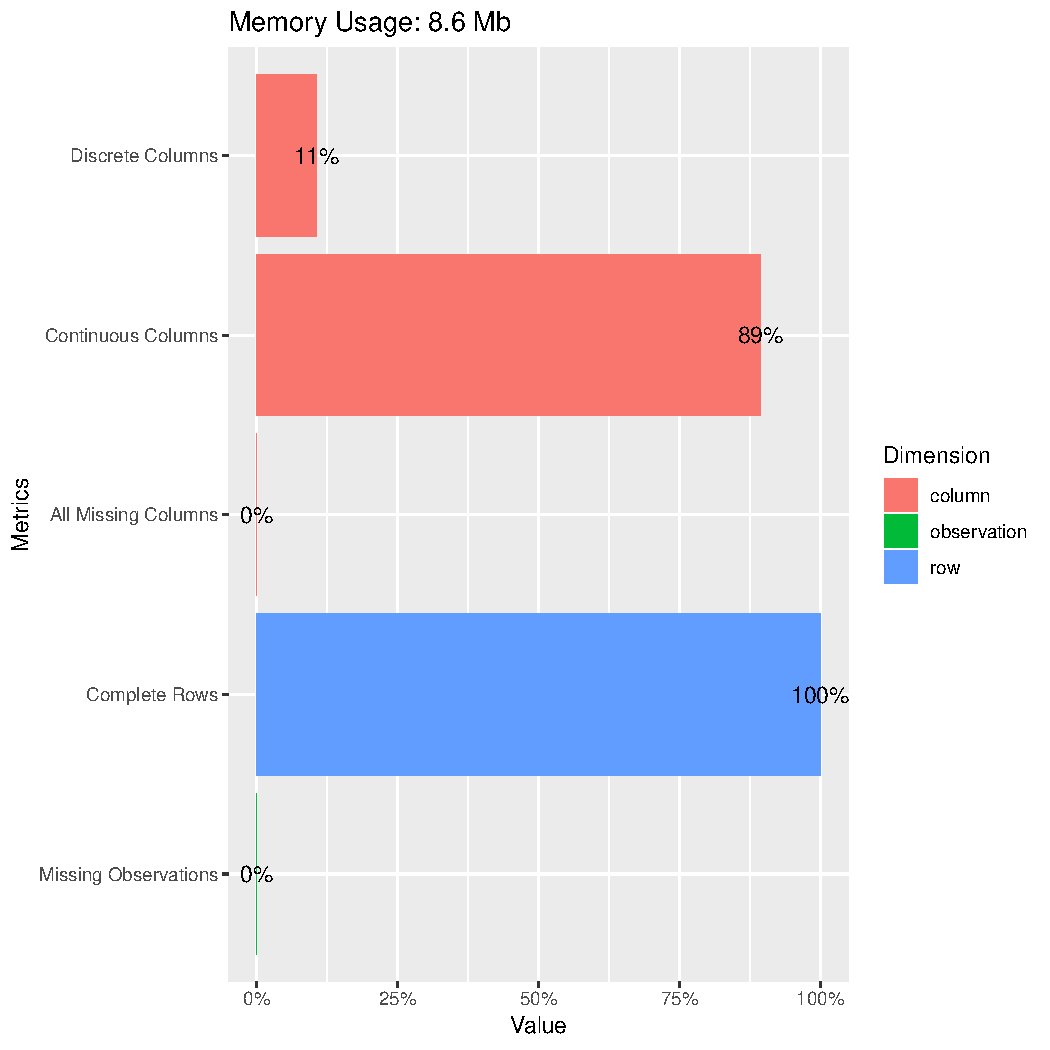
\includegraphics[width=0.5\columnwidth]{images/ml/plot_intro}
	\caption{}
	\label{fig:plot_intro}
\end{figure}

La maggior parte degli attributi del dataset, precisamente 59, sono di tipo 
continuo, mentre solamente 7 sono di tipo discreto. Di tutto il dataset, 
risulta che, in seguito alla selezione degli attributi alla fine del 
procedimento di integrazione, tutte le righe sono complete al 100\%. 

Per andare nel dettaglio di queste variabili, sono stati generati dei diagrammi 
a barre, con la funzione \texttt{plot\_bar}, per quanto riguarda le variabili 
discrete, e gli istogrammi, tramite la funzione \texttt{plot\_histogram}, delle 
variabili continue.

\begin{figure}[htb]
	\begin{subfigure}[t]{1\textwidth}
		\begin{minipage}[t]{.475\textwidth} % not "0.5\textwidth"
			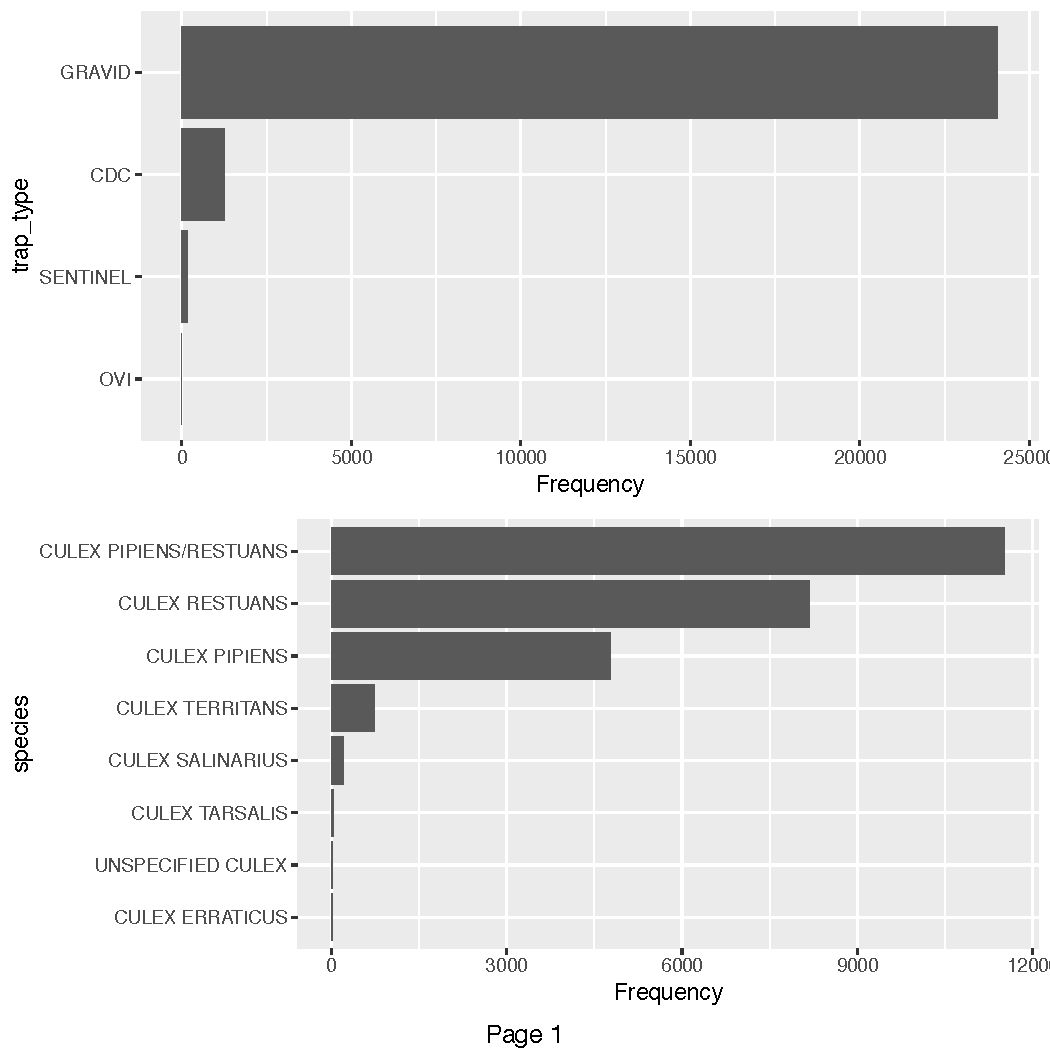
\includegraphics[width=\textwidth]{images/ml/plot_bar1}
		\end{minipage}%
		\hfill
		\begin{minipage}[t]{.475\textwidth}
			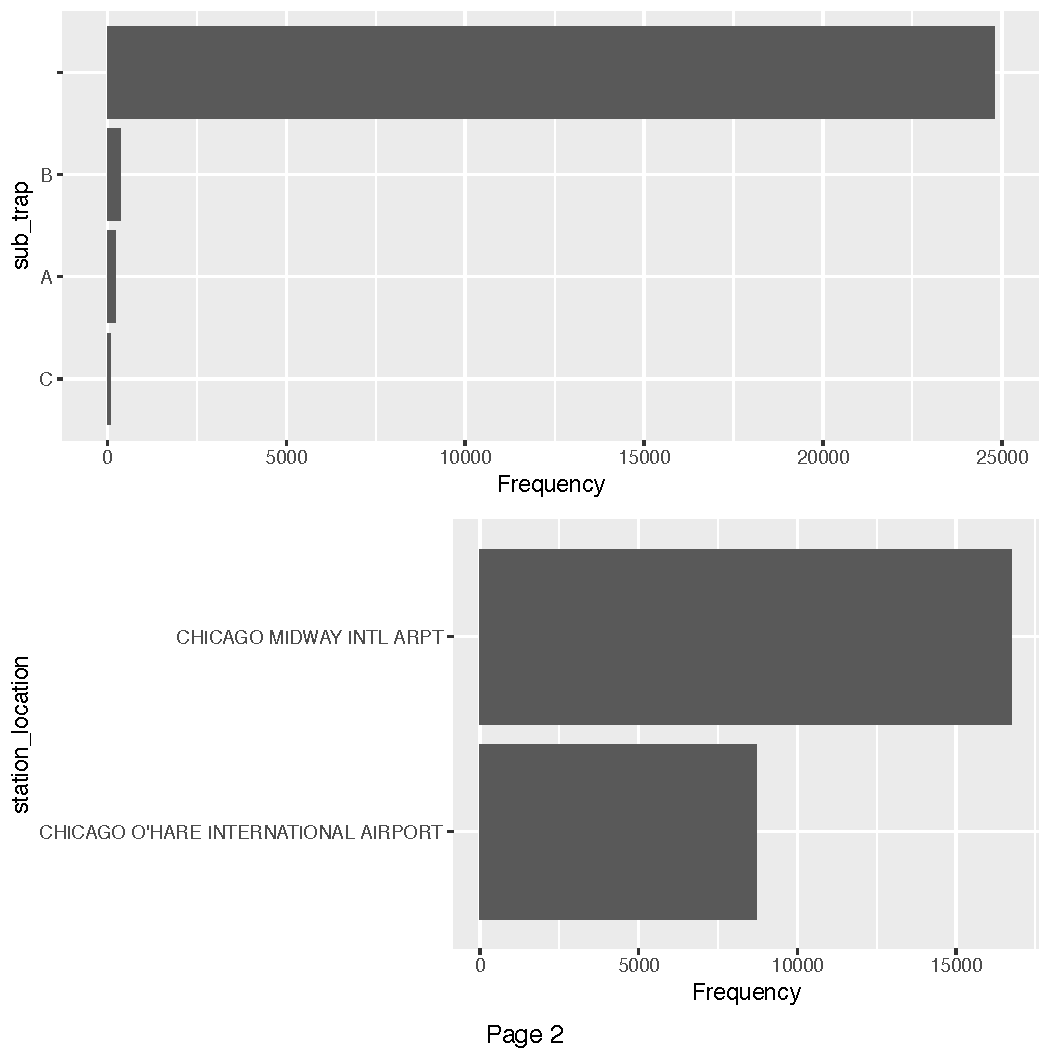
\includegraphics[width=\textwidth]{images/ml/plot_bar2}
		\end{minipage}
	\end{subfigure}
	
	\begin{subfigure}[t]{0.475\textwidth}
	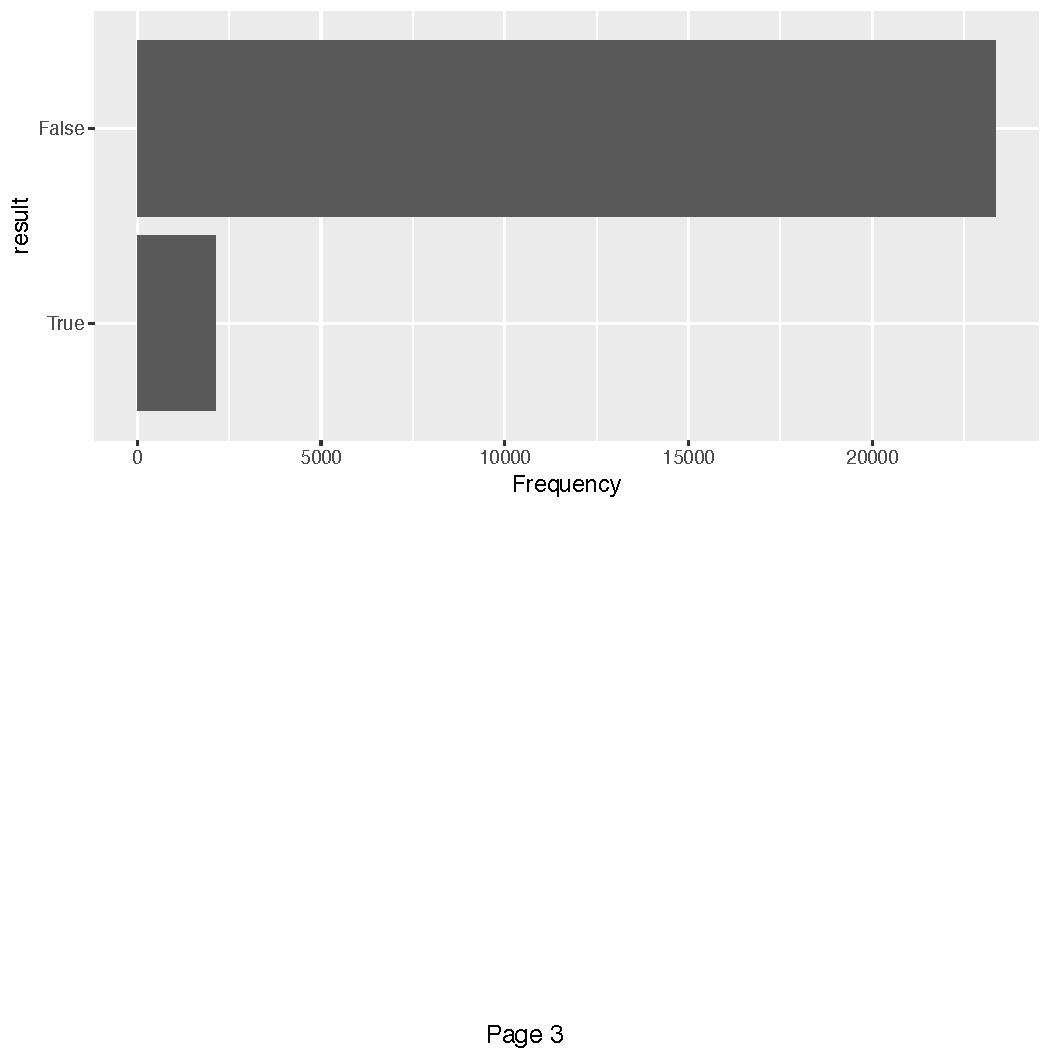
\includegraphics[width=\textwidth]{images/ml/plot_bar3}
	\end{subfigure}
	\caption{GRAFICI bar}
	\label{fig:plot_bar}
\end{figure}

\begin{figure}[htb]
	\centering
	\begin{subfigure}[t]{0.49\textwidth}
		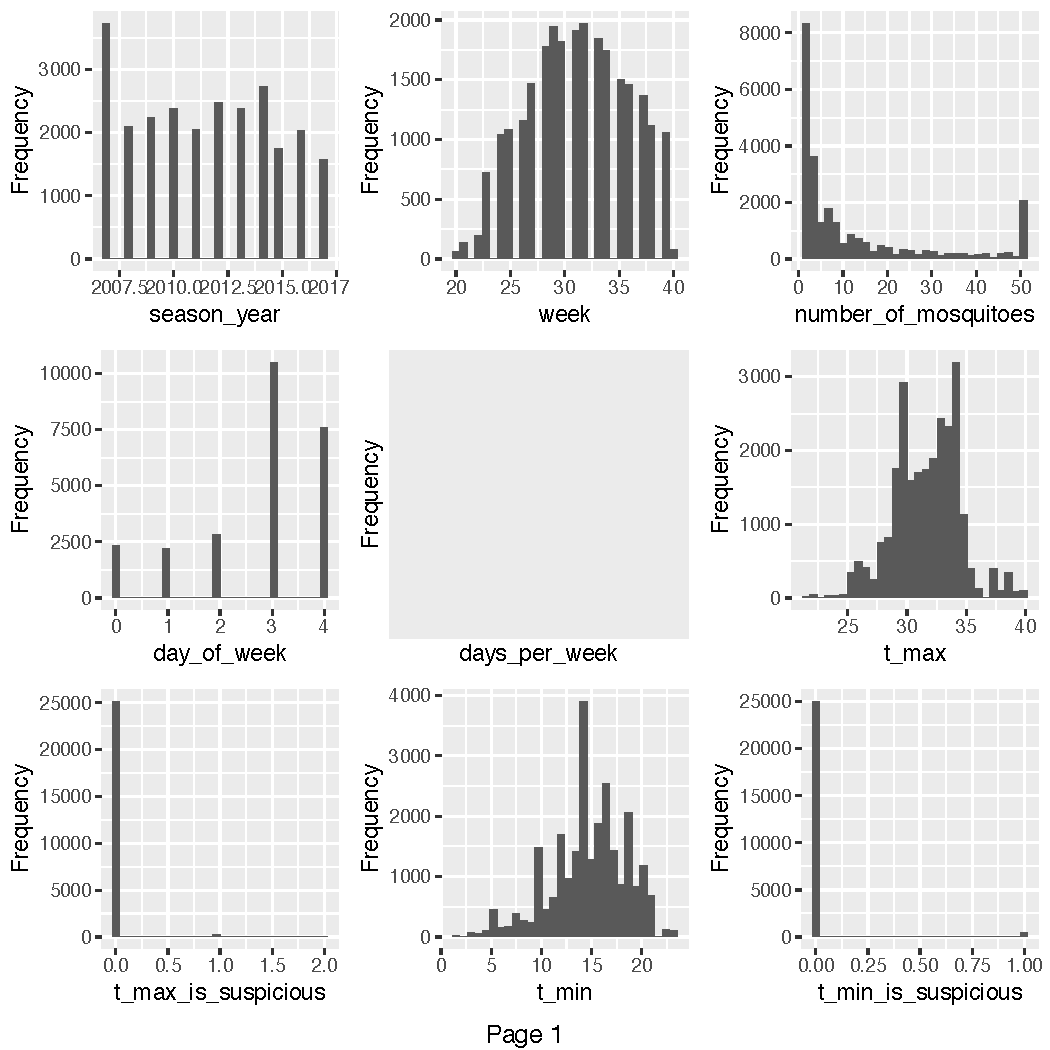
\includegraphics[width=\textwidth]{images/ml/plot_histogram1}
	\end{subfigure}
	\begin{subfigure}[t]{0.49\textwidth}
		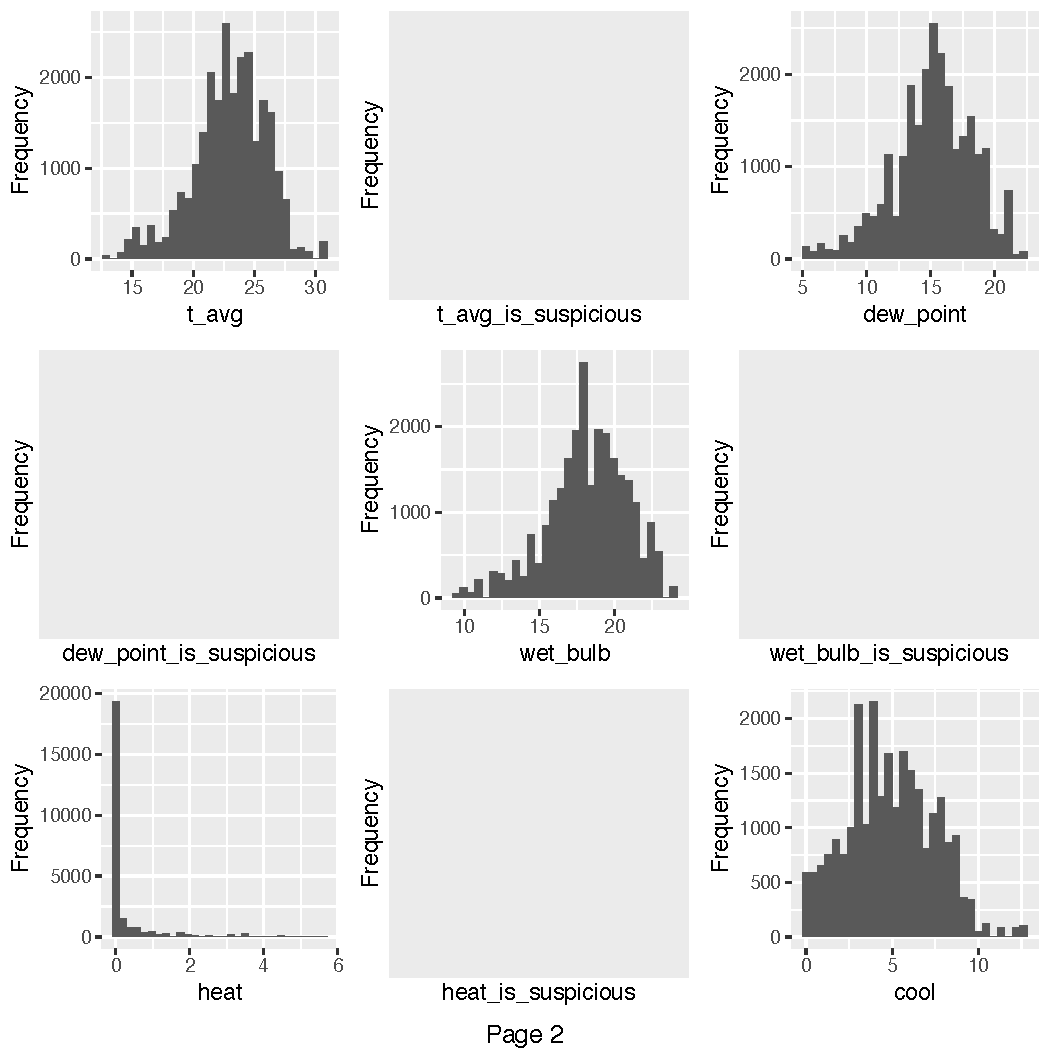
\includegraphics[width=\textwidth]{images/ml/plot_histogram2}
	\end{subfigure}
	\begin{subfigure}[t]{0.49\textwidth}
		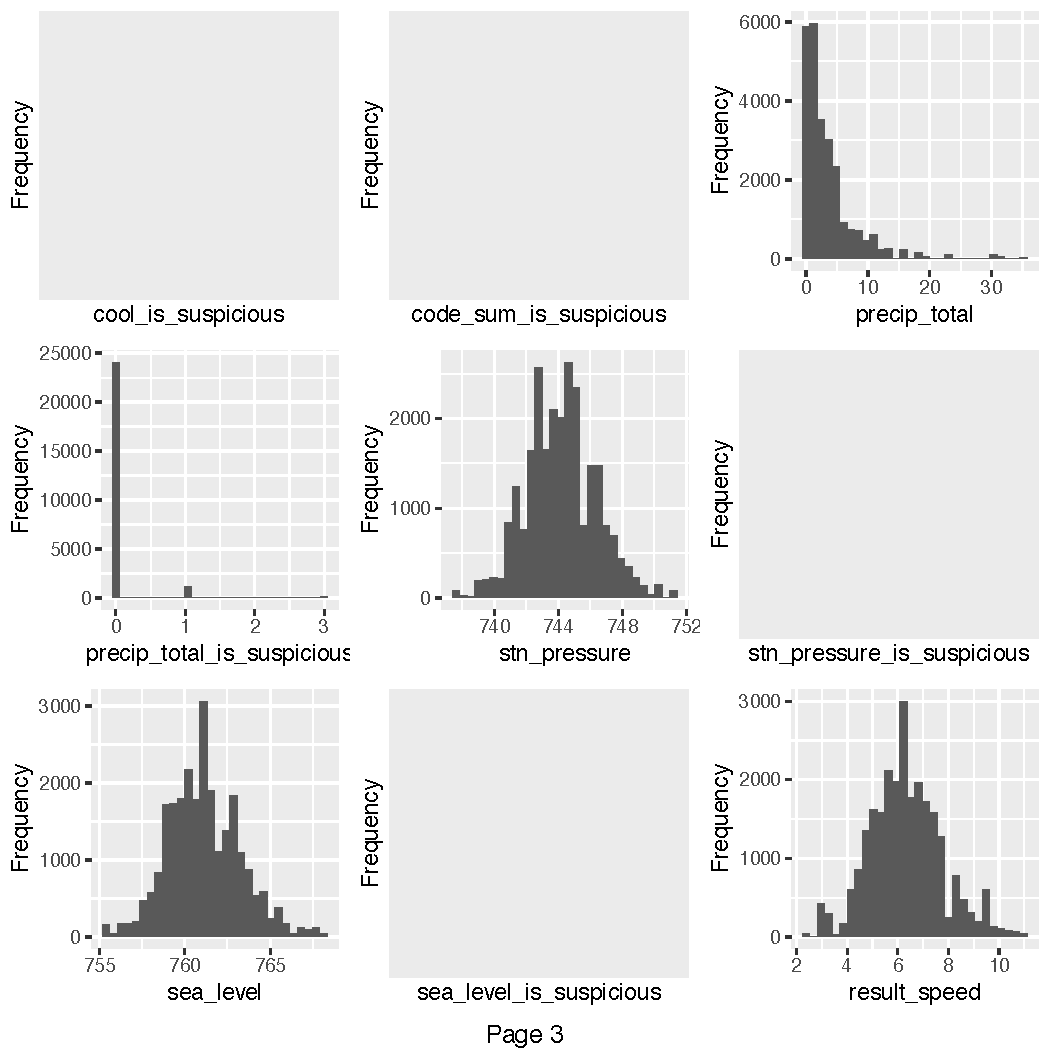
\includegraphics[width=\textwidth]{images/ml/plot_histogram3}
	\end{subfigure}
	\begin{subfigure}[t]{0.49\textwidth}
		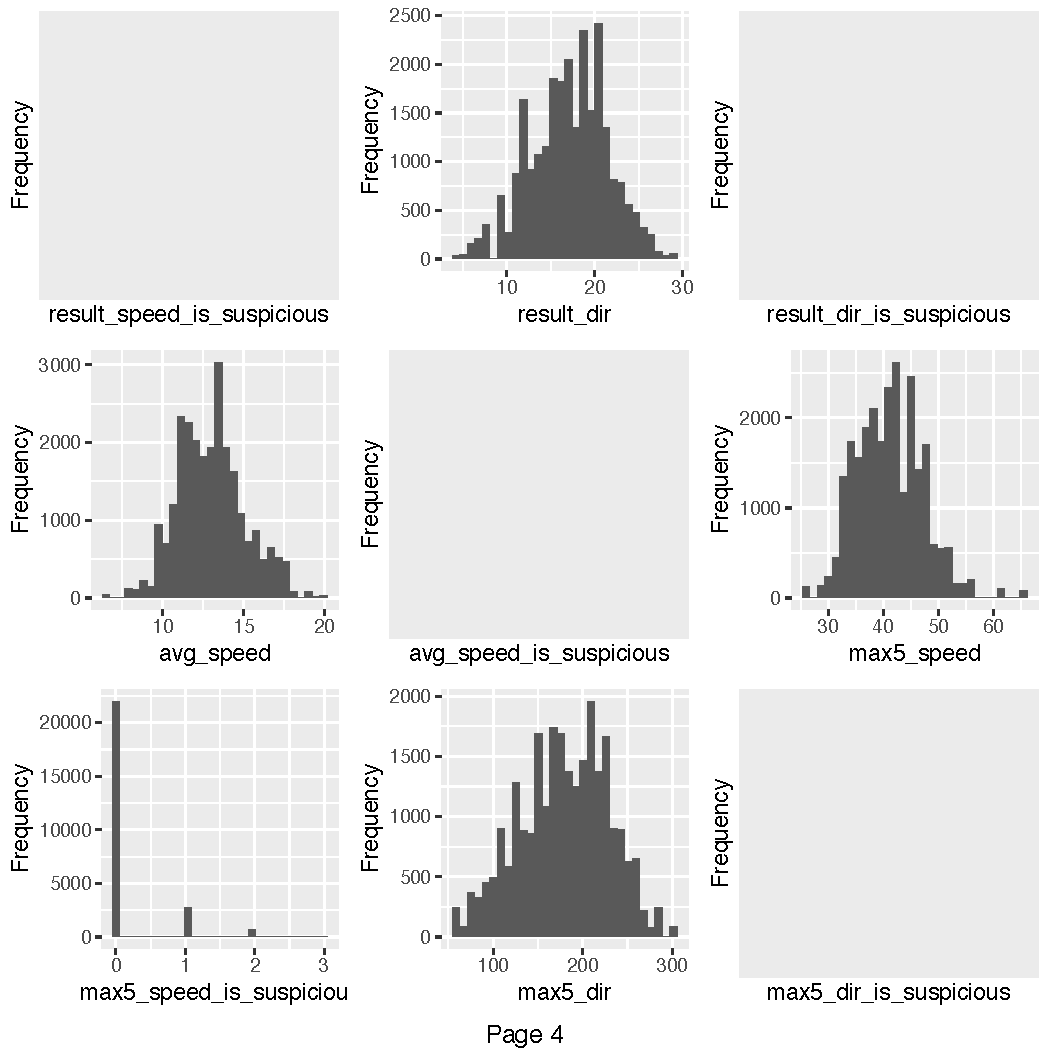
\includegraphics[width=\textwidth]{images/ml/plot_histogram4}
	\end{subfigure}
\end{figure}
\begin{figure}
	\ContinuedFloat 
	\begin{subfigure}[t]{0.49\textwidth}
		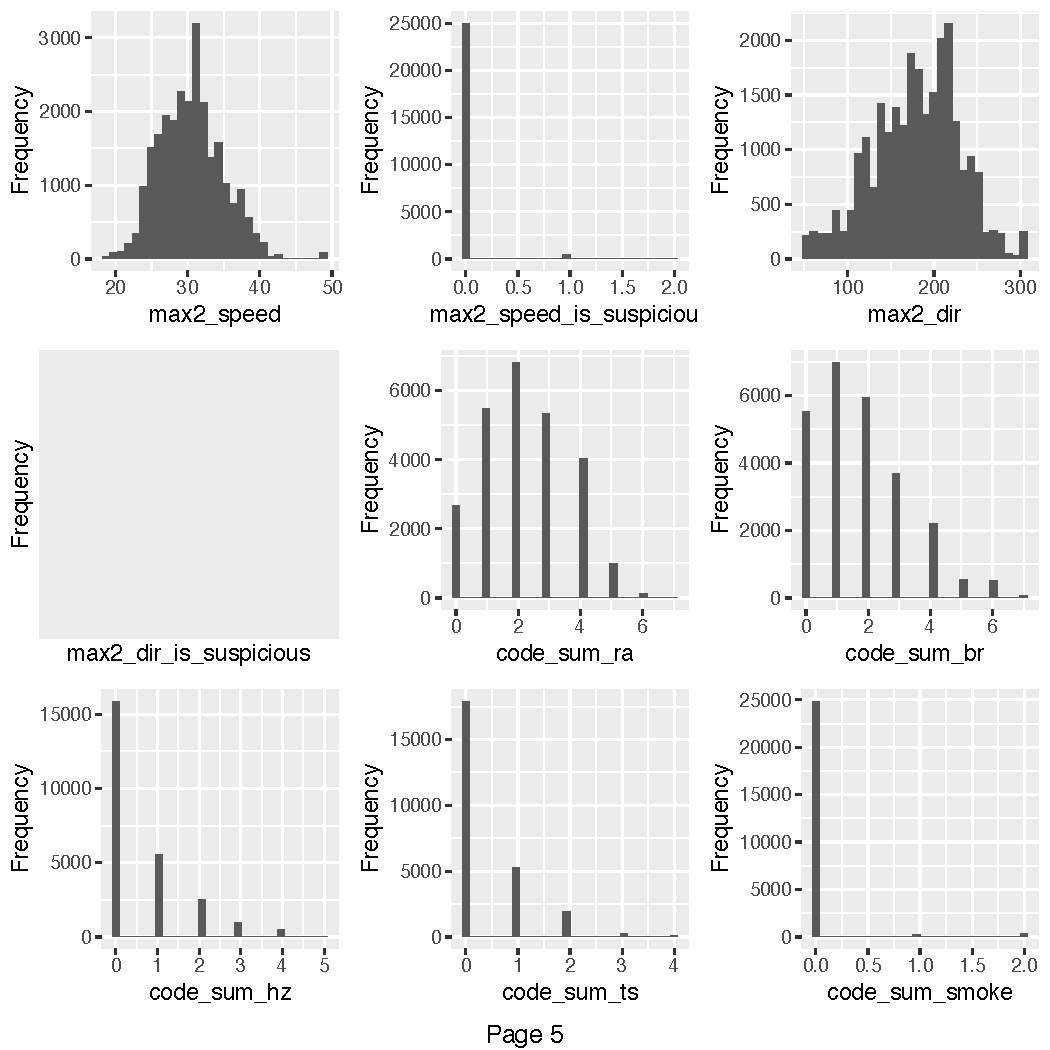
\includegraphics[width=\textwidth]{images/ml/plot_histogram5}
	\end{subfigure}
	\begin{subfigure}[t]{0.49\textwidth}
		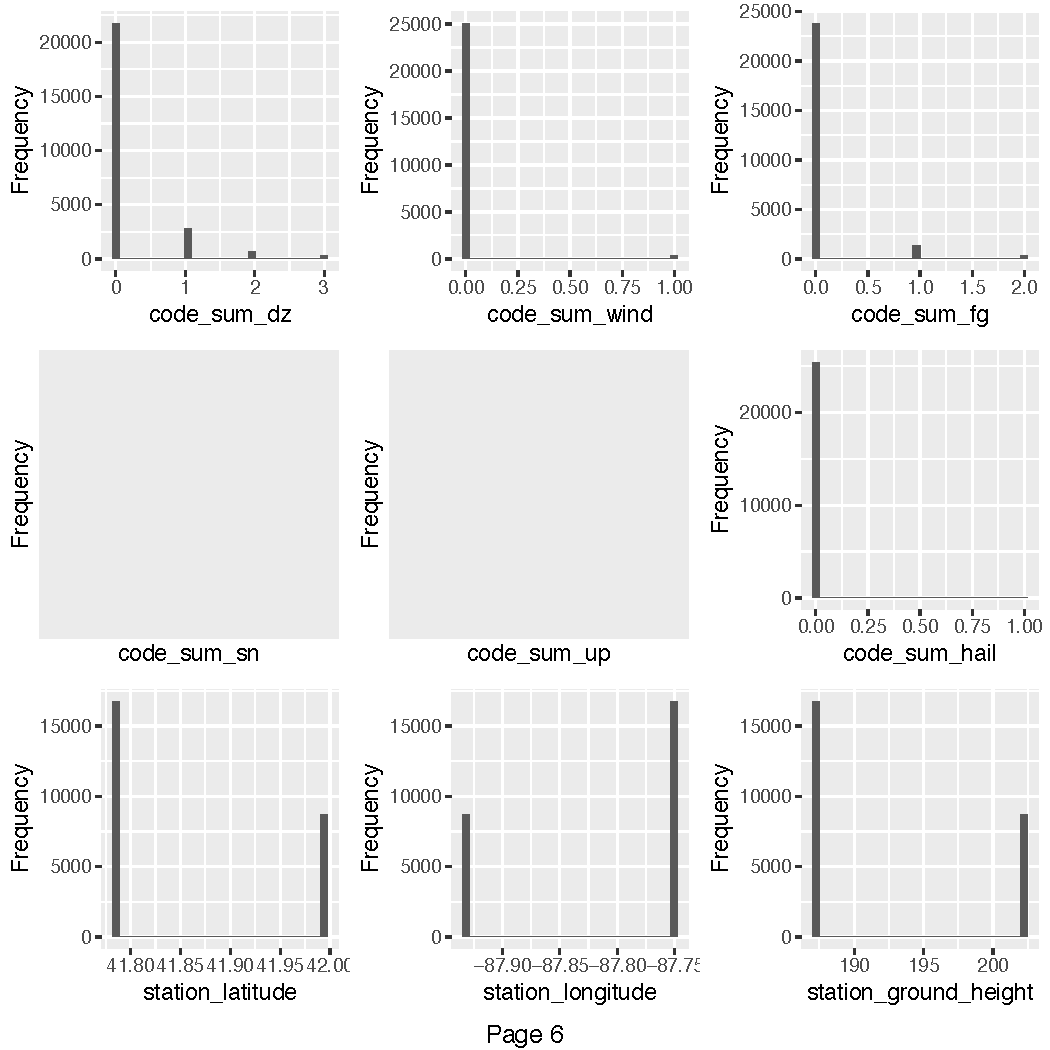
\includegraphics[width=\textwidth]{images/ml/plot_histogram6}
	\end{subfigure}
	\begin{subfigure}[t]{0.49\textwidth}
		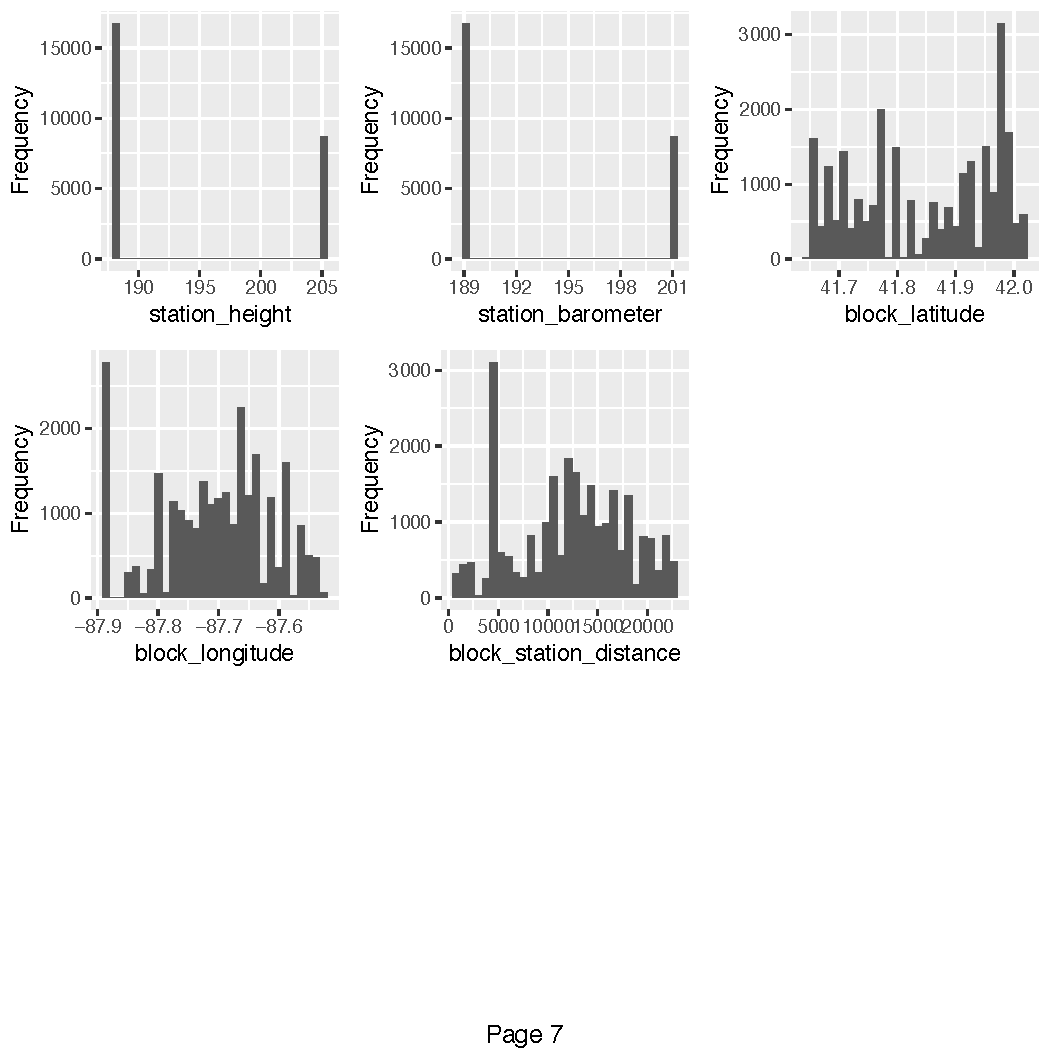
\includegraphics[width=\textwidth]{images/ml/plot_histogram7}
	\end{subfigure}

	
\caption{GRAFICI istogramma}
\label{fig:plot_histogram}
\end{figure}

Da questa analisi si evince che ...
% distribuzione delle variabili, 


In seguito, per evidenziale eventuali correlazioni tra le variabili del 
dataset, è stata visualizzata una matrice di correlazione, grazie la funzione 
\texttt{plot\_correlation}.

% matrie di correlazione generate, dei discreti e dei continui
In figura \ref{fig:plot_correlation} viene mostrato il risultato.

\begin{figure}[htb]
	\centering
	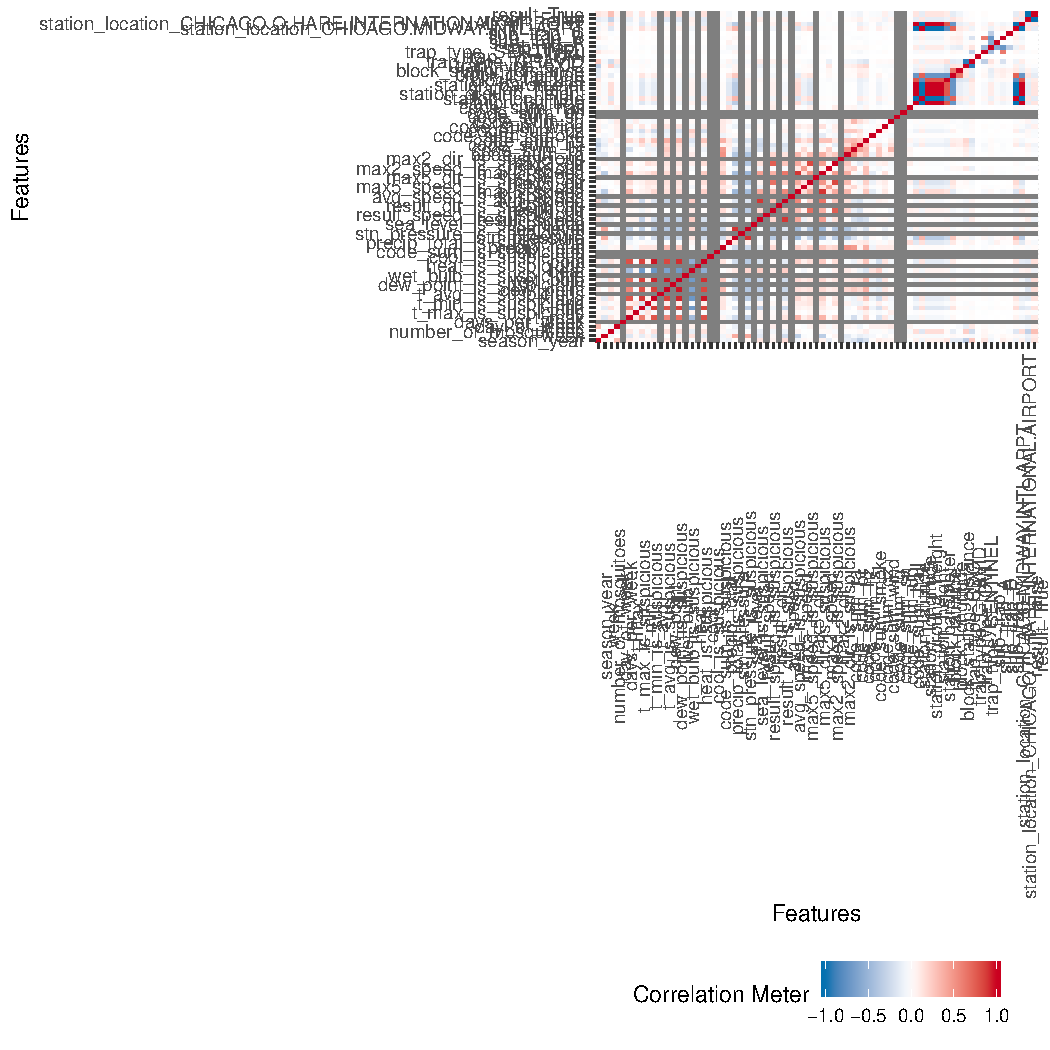
\includegraphics[width=0.5\columnwidth]{images/ml/plot_correlation}
	\caption{}
	\label{fig:plot_correlation}
\end{figure}

Nell'analisi di questa matrice poniamo particolare attenzione alla variabile 
\texttt{result}, ovvero il target del nostro modello.
% analisi...
